%%%%%%%%%%%%%%%%%%%%%%%%%%%%%%%%%%%%%%%%%
% Simple Sectioned Essay Template
% LaTeX Template
%
% This template has been downloaded from:
% http://www.latextemplates.com
%
% Note:
% The \lipsum[#] commands throughout this template generate dummy text
% to fill the template out. These commands should all be removed when 
% writing essay content.
%
%%%%%%%%%%%%%%%%%%%%%%%%%%%%%%%%%%%%%%%%%

%----------------------------------------------------------------------------------------
%	PACKAGES AND OTHER DOCUMENT CONFIGURATIONS
%----------------------------------------------------------------------------------------

\documentclass[12pt]{article} % Default font size is 12pt, it can be changed here

\usepackage{geometry} % Required to change the page size to A4
\geometry{a4paper} % Set the page size to be A4 as opposed to the default US Letter

\usepackage{graphicx} % Required for including pictures

\usepackage{float} % Allows putting an [H] in \begin{figure} to specify the exact location of the figure
\usepackage{wrapfig} % Allows in-line images such as the example fish picture
\usepackage{hyperref}
\usepackage{lipsum} % Used for inserting dummy 'Lorem ipsum' text into the template

\linespread{1.2} % Line spacing

%\setlength\parindent{0pt} % Uncomment to remove all indentation from paragraphs

\graphicspath{{Pictures/}} % Specifies the directory where pictures are stored

\begin{document}

%----------------------------------------------------------------------------------------
%	TITLE PAGE
%----------------------------------------------------------------------------------------

\begin{titlepage}

	\newcommand{\HRule}{\rule{\linewidth}{0.5mm}} % Defines a new command for the horizontal lines, change thickness here

	\center % Center everything on the page


	\textsc{\LARGE Hochschule Düsseldorf}\\[1.5cm] % Name of your university/college
	\textsc{\Large Dokumentation Escape Room}\\[0.5cm] % Major heading such as course name
	\textsc{\large Erweitern und Verändern des bestehenden Raumes}\\[0.5cm] % Minor heading such as course title

	\HRule \\[0.4cm]
	{ \huge \bfseries Dokumentation Escape Room}\\[0.4cm] % Title of your document
	\HRule \\[1.5cm]

	\begin{minipage}{0.4\textwidth}
		\begin{flushleft} \large
			\emph{Autorin:}\\
			Cara \textsc{Watermann} % Your name
		\end{flushleft}
	\end{minipage}
	~
	\begin{minipage}{0.4\textwidth}
		\begin{flushright} \large
			\emph{Supervisor:} \\
			Dr. Christian \textsc{Geiger} % Supervisor's Name
		\end{flushright}
	\end{minipage}\\[4cm]

	{\large \today}\\[3cm] % Date, change the \today to a set date if you want to be precise

	%\includegraphics{Logo}\\[1cm] % Include a department/university logo - this will require the graphicx package

	\vfill % Fill the rest of the page with whitespace

\end{titlepage}

%----------------------------------------------------------------------------------------
%	TABLE OF CONTENTS
%----------------------------------------------------------------------------------------

\tableofcontents % Include a table of contents

\newpage % Begins the essay on a new page instead of on the same page as the table of contents 

%----------------------------------------------------------------------------------------
%	INTRODUCTION
%----------------------------------------------------------------------------------------

\section{Einleitung} % Major section

Die ist eine Dokumentation zum hinzufügen, verändern und erweitern des Escape-Rooms. 
Der erste Teil der Dokumentation widmet sich einer Bestandsaufnahme. 
Teil 2 zeigt, wie der Raum verändert werden könnte. 
Teil 3 handelt von Fehlern, die beim Bauen von Rätseln auftauchen können, und wie sie behoben werden können.


%----------------------------------------------------------------------------------------
%	1. Bestandsaufnahme
%----------------------------------------------------------------------------------------

\section{Bestandsaufnahme} % Major section

Dieses Kapitel soll ein Grundverständnis für die Kommunikation und Vernetzung innerhalb des Raumes erzeugen.

%------------------------------------------------

\subsection{Netzwerk} % Sub-section

Das Netzwerk im Escape-Room besteht im physischen aus 4 Ebenen: \\
Mikrocontrollern (Stand Oktober 2018: Arduino Unos), die mit einem Funkmodul (RFM69HCW) ausgestattet sind.
Über das Funkmodul werden Daten an einen Basis-Microcontroller geschickt (Adafruit 32u4), der wiederrum seriell an den PC angeschlossen ist. 
Vom PC aus können ein Webserver und Unity gestartet werden. 
Mit dem Webserver kann man über das lokale Netzwerk des PCs aktuelle Infos des Pcs bekommen und einzelne Rätseldaten verändern.

\begin{figure}[H] % Example image
	\center{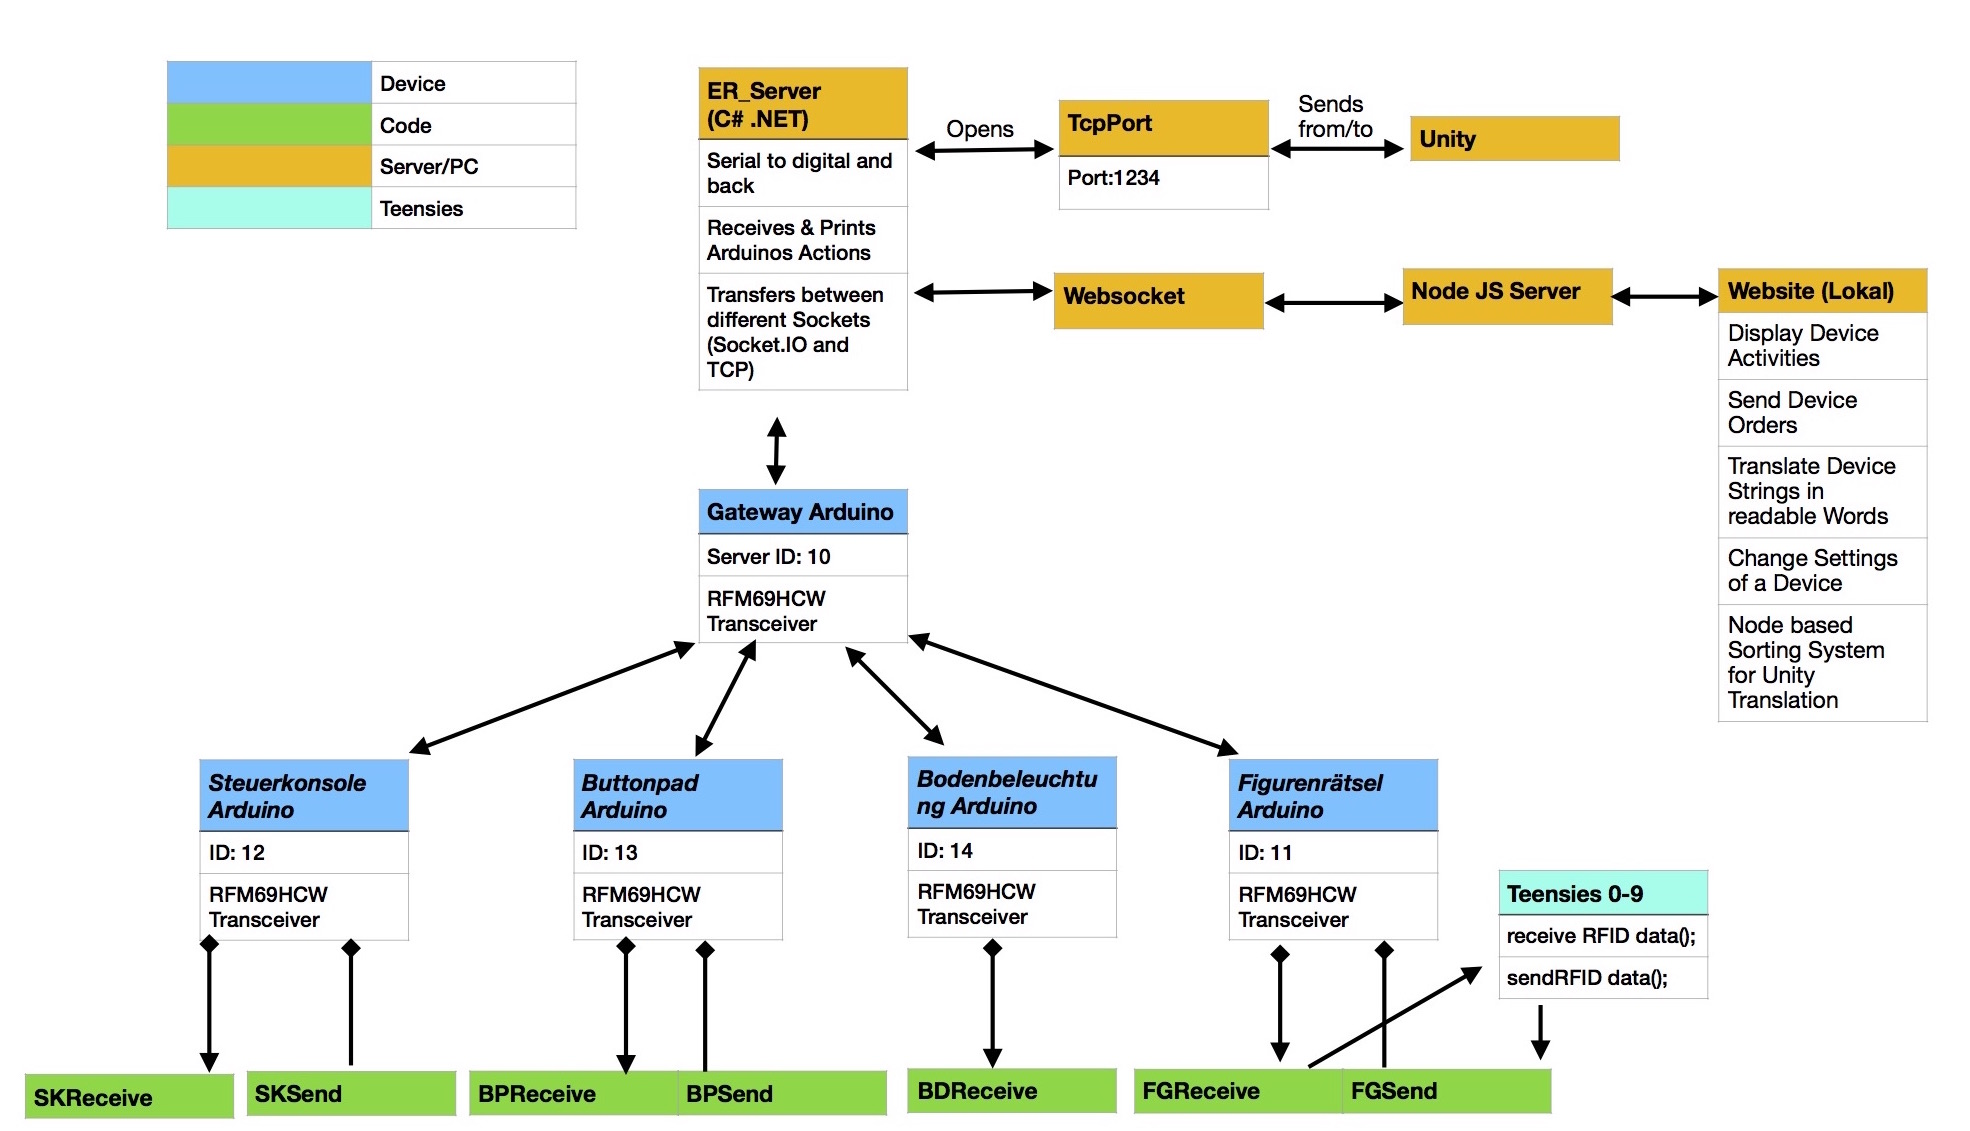
\includegraphics[width=1\linewidth]{escapeuml}}
	\caption{Escape Room UML}
	\label{fig:escape}
\end{figure}

\subsection{Rätsel} % Sub-section

Momentan gibt es 4 Rätsel im Raum, von dem 3 vorgesehenermaßen ein Video in Unity durch triggern bestimmter Codes in Unity starten und pausieren.
Das erste Rätsel (Steuerkonsole) nimmt hierbei eine Sonderrolle ein, da es das Video 3 mal anhalten und starten lässt. 
Zudem gibt es einen LED-Kopf und Bodenbeleuchtung, die von Unity Befehle bekommen wenn das Unity einen bestimmten Triggercode erhält.

%------------------------------------------------

%----------------------------------------------------------------------------------------
%	2. Erweitern und Verändern
%----------------------------------------------------------------------------------------

\section{Erweitern und Verändern}

\subsection{Rätsel} % Sub-section

Im momentanen Zustand des Raumes ist davon auszugehen, dass die meisten zukünftigen Rätsel mit einem Microcontroller und einem Funkmodul ausgestattet sein werden. 
Um diese Rätsel zu programmieren, eignet sich die Arduino IDE. Die folgenden Hinweise eignen sich für Rätsel die mithilfe der "Escape.ino" Datei ein eigenes Rätsel aufbauen wollen.
Der Code für ein neues Rätsel ist in verschiedene Abschnitte eingeteilt. Im Folgenden wird auf die Abschnitte und ihre Bedeutung eingegangen.


\subsubsection{Groundwork}

Im "Groundwork" Teil der "Escape.ino" sollten die benötigten Libaries eingebunden und alle für den Remote und Rätselpart der Anwendung benötigten Variablen definiert werden. 
Einige Variablen werden für jedes Rätsel benötigt und müssen jeweils angepasst werden. Einen Sonderfall spielt hierbei die "NodeID".
Sie definiert die Zahl, über die das Rätsel vom Sender erkannt wird. Für jedes neue Rätsel muss geguckt werden, welche IDs bereits vorhanden sind (siehe Weboberfläche) und eine neue gewählt werden. 
Außerdem sollte alle Variablen einen hier definierten Standardwert haben, falls die Funkverbindung nicht funktioniert, damit das Rätsel auch im Falle von Kommunikationsfehlern bedienbar ist. Bsp.:

\begin{figure}[H] % Example image
	\center{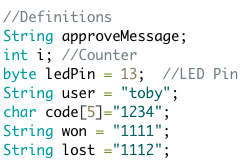
\includegraphics[width=0.5\linewidth]{definitions}}
	\caption{Startwerte der Strings für die registerID}
	\label{fig:def}
\end{figure}

\subsubsection{Riddlefunctionality}
Hier wird die setup() und die loop() funktion initialisiert, sowie alle weiteren Funktionen die direkt mit dem Rätsel zusammenhängen. 
Dieser Abschnitt sollte komplett unabhängig von den folgenden sein und auch ohne Funkverbindung reibungslos ablaufen.


\subsubsection{Remote Functionality}
In diesem Abschnitt sollten alle Kommunikationsfunktionen definiert werden. In "Escape.ino" sind zwei für jedes Rätsel relevante Funktionen vordefiniert: "registerRiddle()" und "remoteCommand()". \\
In "registerRiddle" sollten alle für die Weboberfläche relevanten Nachrichten definiert werden. Hierbei wird zwischen "readonly" und "write" unterschieden, damit die Weboberfläche zwischen statischen und veränderbaren Variablen unterscheiden kann. 
Wenn eine Variable auf "readonly" gesetzt wird, ist nur nötig, ihr einen Titel und den Link zur Variablen zu schicken, damit sie als solche erkannt werden kann. Wenn eine Variable auf "write" gesetzt wird, muss zusätzlich ein Weg zurück zum Microcontroller angegeben werden. Das Pattern ist hierbei "0/CaseNumber/". Die Funktion wird nur aufgerufen, wenn der Standardwert von "startriddle" nicht bereits überschrieben wurde.
Wird eine Variable auf "write" gesetzt, erscheint in der Weboberfläche ein Button zum verändern der Variable. Wird die Variable in der Weboberfläche verändert, wird der neue Wert an den Microcontroller gesendet. \\
In "remoteCommand()" sollte definiert werden, was mit dem verändertem Wert passieren soll. 
Mit einer Switch-Case-Formulierung kann man so direkt auf die in der registerID definerten Werte zugreifen. 
Der Index bestimmt hierbei den Case. Die folgenden Bilder geben ein Beispiel für die registerID "3/write/code/123" an.
\begin{figure}[H] 
  \center{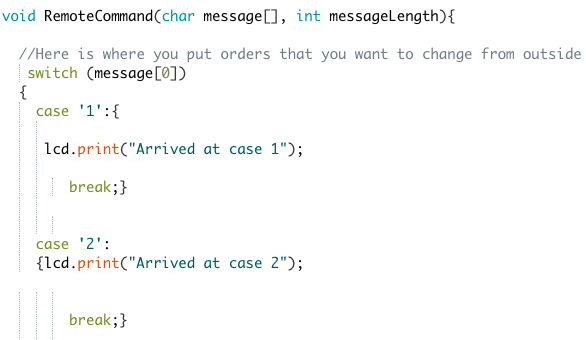
\includegraphics[width=0.5\linewidth]{remotecommand}}
  \caption{Allgemeiner Aufbau der remoteCommand Funktion}
  \label{fig:remoteCommand}
\end{figure}

\begin{figure}[H]
  \center{\includegraphics[width=0.5\linewidth]{sendCode}}
  \caption{Bsp: Änderung des Codes von der Weboberfläche durch "write" Feld}
  \label{fig:sendCode}
\end{figure}

\begin{figure}[H]
  \center{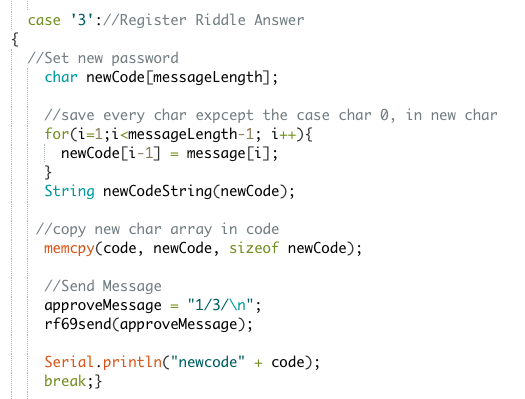
\includegraphics[width=.5\linewidth]{remotecommand2}}
  \caption{Bsp: Arduinoprogrammierung}
  \label{fig:arduino}
\end{figure}
\subsubsection{Radio Functionality}
Der Abschnit "Radio Functionality" behinhaltet die Sender und Empfängerlogik. Sofern die Daten als Strings gesendet werden sollen und ins existierende Schema passen, muss hier nichts verändert werden. 
Sollten die Daten anders verarbeitet werden, können sie von dem Server im momentanen Zustand nicht interpretiert werden.

%------------------------------------------------

\subsection{Weboberfläche} % Sub-section
Die Weboberfläche ist in ein node.js Backend und einen React-Client im Front-End aufgeteilt. 

\subsubsection{Back-End}
Node.js ist JavaScript-Laufzeitumgebung dich sich besonders gut für Webserver eignet und sehr verbreitet ist. 
Eine Studie von Stackoverflow ergab, dass es 2017 und 2018 das beliebteste Web-Framework ist. 
Netflix, Uber und Paypal verwenden es für ihre Websites. 
\href{https://insights.stackoverflow.com/survey/2018#technology}{Stackoverflow}

Die Ordnerstruktur ist orientiert sich an einem Modell, welches die Trennung der Ordner nach Funktion vorschlägt.
Für dieses Projekt gibt es zu momentanen Stand 4 relevante Ordner "db","socket.io", "serial\&tcp" und "test\&info".
Die einzelnen .js Dateien beinhalten jeweils einen Kommentar am Anfang der die Funktion des Komponenten beschreibt.
Abgesehen davon gibt es noch den "client" Ordner der den Veränderbaren Stand des Front-Ends beinhaltet, und den "build" Ordner der den aktuellen build des Front-Ends beinhaltet.
Sobald das Front-End angepasst wurde, kann der build sehr einfach ausgetauscht werden (s. Kapitel Front-End).


\subsubsection{Front-End}
React ist eine von Facebook entwickelte Javascript-Libary, die das zusammenarbeiten von HTML und Javascript flüssig verbindet.
Statt in getrennten Dateien, befindet sich hier alles in einer Javascript-Datei. 
Auch CSS Werte lassen sich hier festlegen, bei größeren Aufwendungen sollten diese jedoch ausgelagert werden.
Damit man die Übersicht nicht verliert, werden hier alle Funktionen in Komponenten aufgeteilt. 

Das hat den großen Vorteil, 
dass man Komponenten relativ einfach in anderen Projekten wiederverwenden kann, und beim Verwenden mehrerer Objekte des gleichen Typs (z.b. 10 Textfelder die auf einen Klick reagieren) der Rechner nur einmal den Komponenten berechnen muss (Textfeld mit Funktion), 
und sonst nur die Variablen (z.b. Textinhalt) neu berechnet. 
Es liest sich nicht genau so wie Javascript und hat einige Besonderheiten (props, states), die auf der React-Seite \href{https://reactjs.org/docs/hello-world.html}{React-Dokumentation}selber gut dokumentiert sind.
Das Front-End wurde mit "Create-React-App" aufgesetzt. 
Daher läuft es mit Babel und Webpack im Hintergrund, und hat eine moderne und standartisierte Struktur.
unter src/Components befinden sich alle fürs Front-End relevanten Komponenten.
Die Benennung ist hoffentlich logisch. 
Wenn das Projekt weiter wächst, macht es Sinn mehr Unterordner einzuführen für die jeweiligen Darstellungen und ihre Komponenten. 
Zum aktuellen Stand sollte das Projekt noch übersichtlich genug gestaltet sein um gut einsteigen zu können.
Am Anfang jedens Komponenten steht in den Kommentaren sein Verwendungszweck. 
In App.js werden sie zusammengefasst und gerendert.
In Index.js wird App.js gerendert, und Bootstrap (CSS Libary) initalisiert. 
In index.css können eigene CSS Änderungen ergänzt werden.
In Components/Sketches können und sollten noch nicht fertige Komponenten gelagert werden, bis sie Produktionsreif sind, damit keine Verwirrung entsteht welche Komponenten fertig sind und welche nicht.
Die grundsätzliche Kommunikation zwischen Front- und Back-end findet via Socket.io, einem Websocket verwendendem Open-Source Projekt statt.
Die Socket.io Events sind nach ihrem Verwendungszweck benannt und triggern wiederrum im Back-End in der Regel eine Datenbankabfrage oder Änderung.
Die meisten Komponenten hören auf Änderungen von der Datenbank. Manchmal muss die Anwendung neu gestartet werden, bevor alle Änderungen richtig dargestellt werden.
Sobald das Front-End geändert wurde, kann es mit "npm run build" im Terminal neu gebaut werden. Dabei handelt es sich um eine komprimierte, effizientere Version des Front-Ends.
Im übergeordnetem Ordner muss dann der alte build ordner durch den neuen ausgetauscht werden. 
Falls das aus Zugriffsgründen nicht möglich ist, funktioniert auch sehr gut die alten Inhalte zu löschen und durch die Inhalte des neuen zu ersetzen.
Das Bild \ref{fig:archFrontend} zeigt nochmal genauer, wie die Einzelnen Komponenten momentan zusammenhängen.

\begin{figure}[H]
	\center{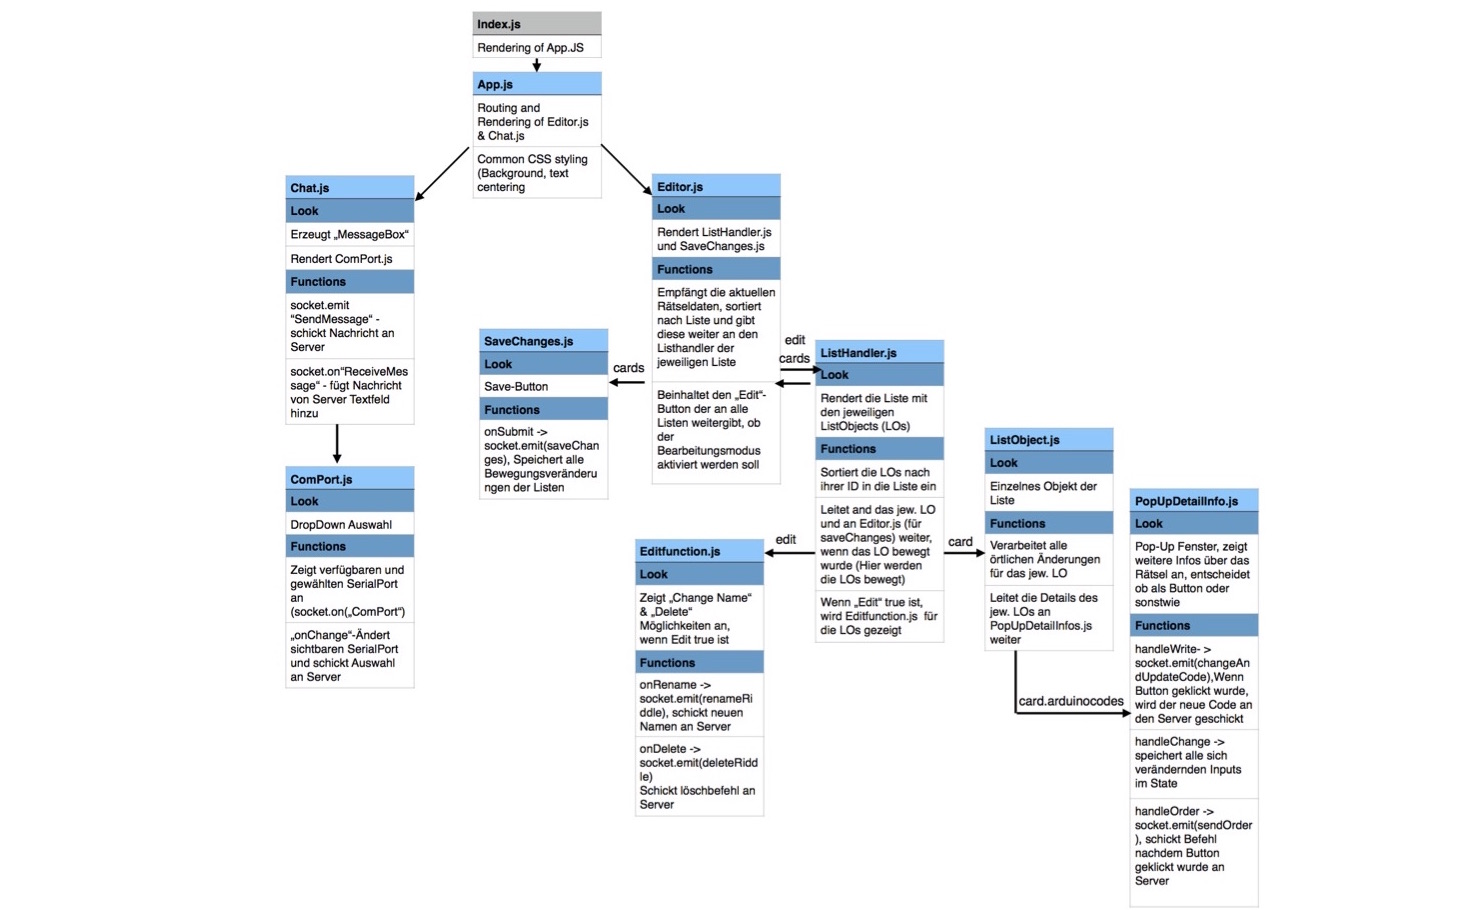
\includegraphics[width=1.2\linewidth]{archFrontend}}
	\caption{Front-End Architektur}
	\label{fig:archFrontend}
  \end{figure}

%------------------------------------------------

\subsection{Unity} % Sub-section

Unity hat im momentanen Zustand einen TCP-Client, der alle Befehle gefiltert entgegen nimmt. 
Das heißt, dass in dem Gateway-Modul abgeglichen wird, welches Rätsel gerade fertig geworden ist (nach einer Codeliste) mit wo es in der Weboberfläche/Datenbank abgespeichert ist.
In Unity selber gibt es mehrere Skripts, die sich mit der Verarbeitung des eingehenden Codes auseinander setzen. 
Es gibt ein Empfängerskript, und pro Rätsel ein Skript welches abgleicht, ob es der dazu passende Startbefehl war.
Falls jemand sich nochmal daran setzten möchte, könnte man hier gut den TCP-Client durch einen Socket.IO Client ersetzen Unityseits, um die Logik komplett von Unity rauszunehmen.
Wie das geht, erkläre ich weiter unten.
Hierfür lediglich die Serialkommunikation und Filterung in node.js nachprogrammiert und dem Webserver hinzugefügt werden.

%------------------------------------------------

\subsection{Set-Up} % Sub-section
Damit wir unser Rätsel starten können, ist hier eine Anleitung zur Integration in den Raum.

Als erstes müssen wir den Raum starten. Dafür müssen folgende Schritte vollzogen werden:

\begin{description} % Numbered list 
	\item[1.] \hfill \\
	      Der Raum muss am Stecker hinten in der Abstellkammer am Ende des Werkraumes eingeschaltet werden.

	\item[2.] \hfill \\
	     Die Steckdosenleiste rechts auf Hüfthöhe in der Klappe muss eingeschaltet werden.

	\item[3.] \hfill \\
		Die beiden PCs müssen hinter der Klappe im Escape Room normal eingeschaltet werden.

	\item[4.] \hfill \\
	      Anschließend sollten alle Devices, die auf den Webserver zugreifen wollen, sich mit dem lokalen W-LAN des Pcs verbinden (Passwort: escape).

	\item[5.] \hfill \\
	      Verbinde dein Rätsel mit einer Stromquelle im Raum oder schalte es ein.
\end{description} % Numbered list 

Nachdem du alle Schritte abgehakt hast, sollte sich dein Rätsel registriert haben und in der Weboberfläche sichtbar sein. Wenn dies nicht der Fall ist, schau im Abschnitt {Bugfixes}.

%----------------------------------------------------------------------------------------
% 3. Fehlersuche
%----------------------------------------------------------------------------------------

\section{Fehlersuche und mögliche Hilfestellungen}



\subsection{Mögliche Projekte für die Zukunft} % Sub-section
\subsubsection{Unity von der Logik trennen}
Wie oben bereits erwähnt, könnte man die unleserlichen Codes von Unity ersetzen durch Socket.io events. Es gibt mehrere Module im Unitystore die Socket.io-client kommunikation ermöglichen.
In Unity müsste mit ein paar Zeilen die man sich auf der Socket.io Seite angucken kann ein Client definiert werden und die enstprechenden Events die das Video abspielen sollen.
Dies würden den Code und den Anpassungsaufwand in Unity immens reduzieren, weil neue Rätsel durch die Weboberfläche die gleichen Events zugeordnet bekommen können wie egal welches Rätsel.
Im Back-End könnte hier in den Emitterfuncs der TCP-Server rausgenommen werden und alle Events, die momentan zu TCP gehen als passende Socket.io Events umgemodelt werden. 
Alle Daten, die Unity an den Serial-Port übertragen werden, würden genau so funktionieren wie die Übertragung ans Web. 
Es macht Sinn einen eigenen Namespace in Socket.io zu erstellen, um die Filterung der Daten (wann was geschickt werden soll) vom Web-empfänger zu unterscheiden.
Der Namespace, gibt vor, dass nur Empfänger die auf diesen Namen hören diese Events bekommen. Momentan gibt es einen Namespace, nämlich web, und den globalen namespace, io. Das heißt Unity würde intuitiv nur die io events kriegen.
Das ist nicht schwer, und wie das geht sieht man in der server.js Datei (Serverseitig) am beispiel des "Web" Empfängers. Wenn die Variable global gemacht wird (auch am Beispiel der Web und io Variablen zu erkennen), kann jede Datei Events emitten.
Empfängerseitig ist das genau so einfach, und am Beispiel der iosetup.jsx Datei im Front-End zu erkennen.

\subsection{Nützliche Links} % Sub-section
Im Folgenden sind Links aufgelistet, die vielleicht weiterhelfen können.

Hier befinden sich alle Architektur Dateien zum Download und verändern:  
\href{https://www.icloud.com/numbers/0841q8aak3co6xR5aNUxTdjNQ#EscapeUML}
Bachelor-Arbeit zur ausführlichen Erklärung der erfoderlichen Konzepte:
\href{https://github.com/reflaxo/BachelorThesisCW/blob/master/main.pdf}
Socket.io Dokumentation
\href{https://socket.io/}
React Dokumentation
\href{https://reactjs.org/}
React Intro-Kurs zum verstehen der Grundprinzipien
\href{https://www.codecademy.com/learn/react-101}
Node.JS Dokumentation
\href{https://nodejs.org/en/docs/guides/}
RFM69HCW Packet-Radio Erklärung/Anleitung zum Verkabeln und Programmieren
\href{https://learn.adafruit.com/adafruit-rfm69hcw-and-rfm96-rfm95-rfm98-lora-packet-padio-breakouts/overview}
LowPowerLab Libary
\href{https://github.com/LowPowerLab/RFM69}{https://github.com/LowPowerLab/RFM69}
%----------------------------------------------------------------------------------------
%	CONCLUSION
%---------------------------------------------------------------------------------------
%----------------------------------------------------------------------------------------
%	BIBLIOGRAPHY
%----------------------------------------------------------------------------------------


%----------------------------------------------------------------------------------------

\end{document}